\section{Introducción a funciones}

%\subsection{¿Qué es una función?}

%Unos de los principales conceptos en álgebra es la función. Hay muchas maneras para describir una función y empezaremos por definir una función como un tipo especial de relación

%\begin{definicion}
%Una relación en que cada coordenada-$x$ es emparejada con solo una coordenada-$y$ se dice que describe $y$ como una función de $x$.
%\end{definicion}

%\begin{ejercicio}
%Cuál de las siguientes relaciones describe $y$ como una función de $x$?

%\begin{enumerate}
    %\item $R_1=\{(-2,1), (1,3), (1,4), (3,-1)\}$
   %\item $R_2=\{(-2,1), (1,3), (2,3), (3,-1)\}$
%\end{enumerate}

%\end{ejercicio}

%\begin{solution}
%\vspace{4cm}
%\end{solution}

%Notar que en el ejercicio anterior, la relación $R_2$ contiene dos puntos diferentes con la misma coordenada en $y$. Recordar, que para decir que $y$ es una función de $x$, solo necesitamos asegurarnos que la misma coordenada en $x$ no fue usada en más de un punto.

%\begin{teorema}[La Prueba de la Línea Vertical]
%Un conjunto de puntos en el plano representa $y$ como una función de $x$ si y solo si caen en la misma linea vertical.
%\end{teorema}


%\begin{ejercicio}
%Use la Prueba de la Linea Vertical para determinar cuales de las siguientes relaciones describe $y$ como una función de $x$.
%\end{ejercicio}

%\begin{figure}
%    \centering
%    \includegraphics[width=0.5\textwidth]{Imagenes/IMG2/Ejercicio.png}
%    \caption{}
%    \label{fig:enter-label}
%\end{figure}

%\begin{solution}
%\vspace{4cm}
%\end{solution}

%Para que no cumpla la Prueba de la Linea Vertical basta con encontrar una línea.

%\begin{definicion}
%Suponga que $F$ es una relación que describe $y$ como una función de $x$

%\begin{itemize}
%    \item El conjunto de coordenadas en $x$ de los puntos en $F$ se llama el \textbf{dominio} de $F$
%   \item El conjunto de coordenadas en $y$ de los puntos en $F$ se llama el \textbf{rango} de $F$
%\end{itemize}
%\end{definicion}

%Todas las funciones son relaciones, pero no todas las relaciones son funciones. La representación algebraica de las funciones es posiblemente la forma más importante de verlas, así que necesitamos un proceso para determinar si una ecuación representa una función.

%\begin{problema}
%Determine cual ecuación representa $y$ como una función de $x$.

%\begin{multicols}{3}
%    \begin{enumerate}
%        \item $x^3+y^2=1$
%        \item $x^2+y^3=1$
%        \item $x^2y=1-3y$
%    \end{enumerate}
%\end{multicols}
%\end{problema}

%\begin{solution}
%\vspace{4cm}
%\end{solution}
En matemáticas y en las ciencias el concepto de función es muy importante, en muchas ocasiones asignamos a cada elemento de algún conjunto un elemento particular de un segundo conjunto. En la vida común hay diversos ejemplos de funciones, desde cuando se hace un simple chequeo médico hasta algún tipo de información u noticia relevante que vemos por los medios de información; por ejemplo en un chequeo médico emparejan nuestros datos junto con datos de temperatura, edad, peso, presión etc, podemos pensar entonces que la enfermera en cuestión tiene un conjunto de todos los pacientes de tal día emparejandos con algún subconjunto de valores que indican la temperatura. En matemáticas discretas las funciones se usan en definiciones de estructuras como sucesiones o cadenas, o como funciones recursivas que se definen en términos de ellas mismas.

\begin{definicion}
    Sean $A$ y $B$ conjuntos. Una función $f$ de $A$ en $B$ es una correspondencia, que asigna a cada elemento de $A$ exactamente un elemento de $B$. Escribimos $f(a)=b$ si $b$ es el único elemento de $B$ que fue asignado mediante $f$ al elemento $a$. Si $f$ es una función de $A$ en $B$ escribimos $f: A \longrightarrow B$.
\end{definicion}

Las funciones pueden definirse de muchas maneras, en cálculo es común trabajar con funciones de números reales en si mismos; es decir, $f: \mathbb{R}\longrightarrow \mathbb{R}$, estas comúnmente se pueden definir mediante una fórmula explícita y entonces se acostumbra a suprimir la notación anterior. Es posible que el estudiante ya tenga una idea de esto; por ejemplo $f(x)=x^2$, es la función que a cada $x \in \mathbb{R}$ le asigna su cuadrado.

\begin{definicion}
    Si $f$ es una función de $A$ en $B$, decimos que $A$ es el dominio de $f$, en otras palabras el dominio son todos los posibles valores que toma $f$ para tranformarlos en elementos del conjunto $B$. Si $f(a)=b$ decimos que $b$ es la imagen de $a$, mientras que $a$ es una preimagen de $b$. Al conjunto $B$ se le conoce como codominio o conjunto de llegada, cabe resaltar que no necesariamente llegamos a recorrer todo el conjunto $B$. El rango o imagen de la función $f$ es el conjunto de todas las imágenes de elementos de $A$ y se denota como $f(A)$, en notación de conjuntos tenemos que $$f(A)=\{\, f(x)\,| \,\,\, x \in A\,\,\}.$$
\end{definicion}

Si pensamos que el dominio de una función es un conjunto de \textbf{entrada/inputs} y el rango un conjunto de \textbf{salida/outputs}, podemos pensar que una función $f$ es un proceso mediante el cual cada entrada $x$ se empareja con solo una salida $y$. Esto lo podemos simbolizar como $f(x)=y$.

\begin{center}
    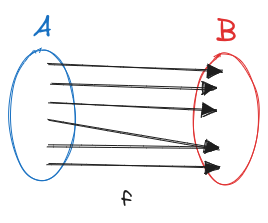
\includegraphics[scale=0.55]{Imagenes/IMG2/S1-2-02.png}
\end{center}

\begin{ejemplo}
Sea $f: \mathbb{N} \longrightarrow \mathbb{N}$, donde la función $f$ le asigna a cada número natural $n$ el número par $2n$. En este caso podemos escribir una regla de correspondencia para $f$; que es $f(n)=2n$, Notemos que el conjunto de llegada es $\mathbb{N}$, sin embargo $f$ no recorre a todos los elementos de este. En este caso el rango de $f$ es el subconjunto de los números pares positivos.
\end{ejemplo}

\begin{ejemplo}
Consideremos el conjunto $P$ formado por Aldo, Carlos, Berenice, Alberto, Elena, Efraín y el conjunto $B$ de los números enteros positivos desde el $1$ al $8$. Sea $\varphi$ la función que a cada nombre de los individios le asigna un número entre el $1$ y $8$, como en la siguiente figura.
\begin{center}
    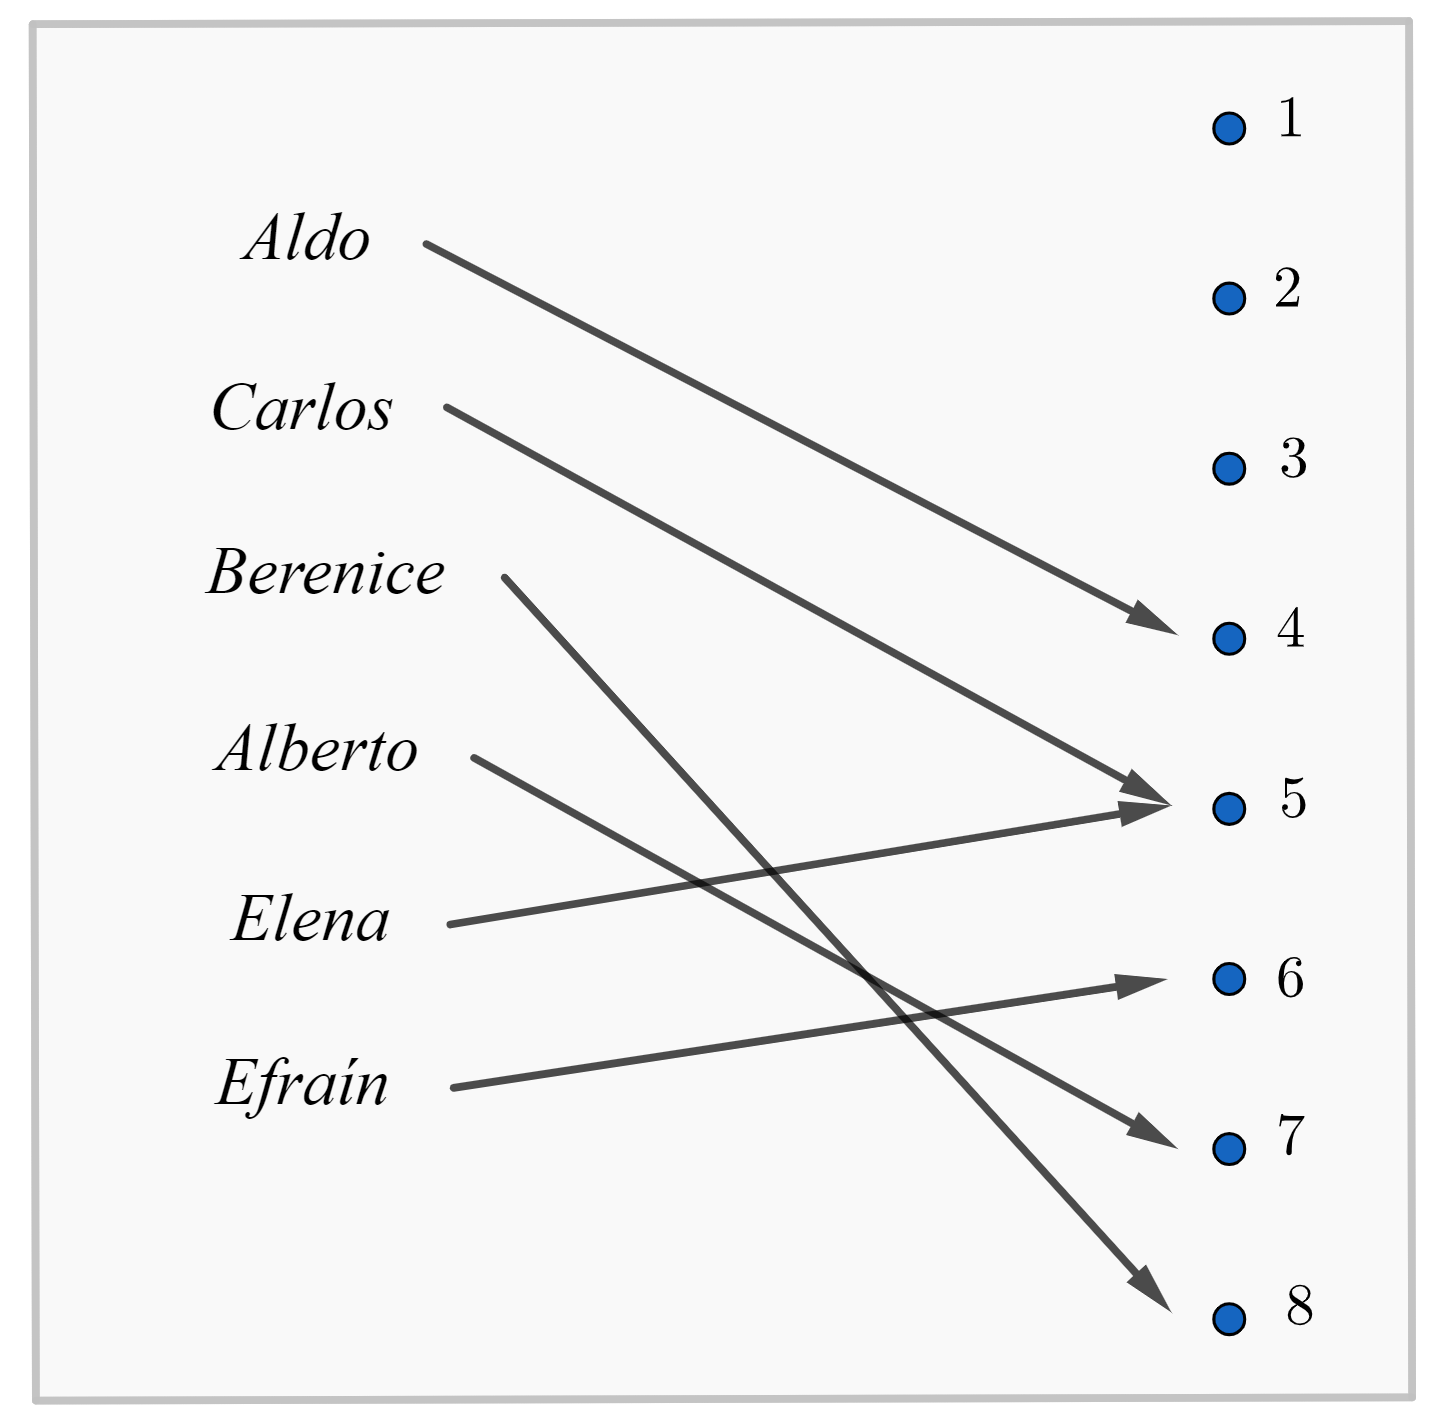
\includegraphics[scale=0.2]{Imagenes/IMG2/S1-2-01.png}
\end{center}

Notemos que la función $\varphi$ asigna el número de letras de cada uno de los nombres, por lo que de alguna manera podemos tener una fórmula para $\varphi$. Notemos también que la función no recorre todos los elementos del conjunto de llegada $B$. El rango de esta función está conformado por los números enteros mayores que 4 y menores a 8.
\end{ejemplo}



\subsection{Inyectividad, biyectividad y sobreyectividad}

\begin{definicion}[Inyectividad]
Una función $f:A\to B$ se dice que es inyectiva si a elementos distintos de su dominio, le asigna imágenes distintas en su rango.
\end{definicion}

Que una función sea inyectiva quiere decir que para cualquier elemento de $B$ solo llega una única flecha a este, en términos más matemáticos:
\begin{center}
    Si $x_1, x_2 \in A$ y $f(x_1)=f(x_2)$, entonces $x_1=x_2$.
\end{center}

\begin{center}
    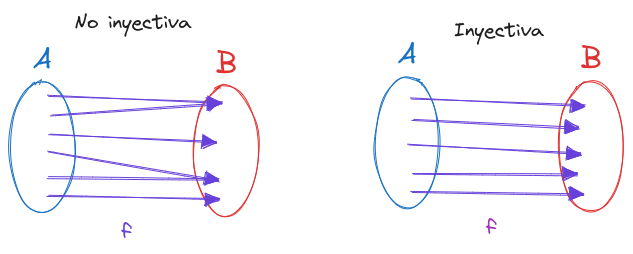
\includegraphics[scale=0.55]{Imagenes/IMG2/S1-2-03.png}
\end{center}

\begin{ejemplo}
Probar que $g : \mathbb{R} \to \mathbb{R}$ definida por $g (x) = x^2$ no es inyectiva
\end{ejemplo}

\begin{solucion}
Para ser inyectiva para cualesquiera par de elementos $x_1, X_2$ que tomemos en el dominio debe verificar que si ${x_1}^2={x_2}^2$, entonces $x_1=x_2$. Pero notemos que con $X_1=1$ y $x_2=-1$, tenemos que $g(-1)=g(1)$, pero $1 \neq -1$.    
\end{solucion}
    

\begin{definicion}[Sobreyectividad]
Una función $f:A\to B$ se dice que es sobreyectiva si $f(A)=B$, es decir, para cada $y\in B$ existe $x\in A$ tal que $f(x)=y$
\end{definicion}

Con estas condiciones la función $g$ definida en el ejemplo anterior no es sobreyectiva; pues no existe $x\in \mathbb{R}$ tal que $x^2=-1$. Tampoco es inyectiva la función del ejemplo 2 de esta sección.


\begin{definicion}[Biyectividad]
Una función $f$ es sobreyectiva si es inyectiva y biyectiva.
\end{definicion}

\section{Principio de correspondencia}

\begin{definicion}
Dos conjuntos $A$ y $B$ se dicen coordinables si existe una función biyectiva $f: A\to B$. En este caso se escrbe $A \cong B$
\end{definicion}

\begin{definicion}
Un conjunto $A$ se dice que es finito si es vacío o si es coordinable con un conjunto de la forma $I_n=\{1,2,3,\dots, n\,\}$ y en este último caso se dice que el cardinal de $A$ es $n$, o bien que el número de elementos que posee es $n$. Cuando $A$ es vacio decimos que el conjunto tiene cero elementos.
\end{definicion}

\begin{problema}
¿Cuántos términos tiene la progresión aritmética $17, 20, 23, 26, \dots, 170$?
\end{problema}

\begin{solucion}
Sea $\varphi : I_{52} \longrightarrow \{17, 20, 23, 26, \dots, 170\}$, dada por $\varphi(n)=17+3(n-1)$, notemos que esta función es biyectiva por lo que el total de términos es $52$.
\end{solucion}

\begin{ejercicio}
¿Cuál es el total de cadenas de ceros y unos de longitud 6? Por ejemplo, la cadena 100010 es de longitud seis.
\end{ejercicio}

\begin{ejercicio}
¿Cual es el número de subconjuntos que posee un conjunto $A$ de cardinal $n$?
\end{ejercicio}

\section{Recurrencia.}

La recurrencia consiste en suponer que se conocen los valores de una función de conteo para todos los valores previos a $n$, luego con esto intentamos determinar a partir de esta información el valor para $n$.

\begin{ejemplo}
¿Cual es el número de subconjuntos que posee un conjunto $A$ de cardinal $n$?    
\end{ejemplo}

\begin{solucion}
Resolvemos este problema usando ahora recursión. Dado un conjunto $A$ de cardinal $n$, supongamos que sabemos cuál es la cantidad de elementos de un conjunto de cardinal $n-1$. Sea $S_{k}$ el total de subconjuntos de un conjunto de cardinal $k$, así $S_{n-1}$ es el total de subconjuntos de un conjunto de cardinal $n-1$. Si $A=\{a_1, a_2, \cdots a_n \}=\{a_1, a_2, \cdots a_{n-1} \}\cup \{a_n\}$, El total de subconjuntos de $A$ puede dividirse como el total de subconjuntos que no continen a $a_n$ y el total de subconjuntos que contienen a $a_n$, así por el principio de la suma $$|A|=|\{\text{subconjuntos que contienen a}\,\, a_n\}|+|\{\text{subconjuntos que no contienen a}\,\, a_n\}|,$$ pero el total de subconjuntos que contienen no contienen a $a_n$ es $S_{n-1}$, mientras que cualquier subconjunto $B\subset A$ que contiene a $a_n$ es de la forma $B=C\cup \{a_n\}$, donde $C$ es un subconjunto de $\{a_1, a_2, \cdots a_{n-1} \}$, por el principio de correspondencia también hay $S_{n-1}$, suconjuntos de $A$ que contienen a $a_n$, por lo tanto $S_n=2S_{n-1}$ y dado que en un conjunto de cardinalidad $1$, solo tiene a los subconjuntos $\emptyset$ y el mismo, sabemos que $S_1=2$, por lo tanto

\begin{eqnarray*}
    S_{n} & = & 2S_{n-1}\\
    & = & 2^2S_{n-2}\\
    & = & 2^3S_{n-3}\\
    & \vdots & \\
    & = & 2^{n-1}S_1=2^n.
\end{eqnarray*}
\end{solucion}

\begin{ejemplo}
    Determinar el número de diagonales de un polígono convexo de $n$ lados.
\end{ejemplo}

\begin{solucion}
    Sea $D_n$ el número de diagonales de un polígono convexo de $n$ lados, sabemos que $D_4=2$. Para definir una función de recurrencia, imaginemos que un polígono de $n$ lados podemos obtenerlo a partir de un polígono de $n-1$ lados tomando uno de los vértices, abriendo la figura para introducir un nuevo vertice a luego cerrando los segmentos, como en la figura siguiente:
    \begin{center}
        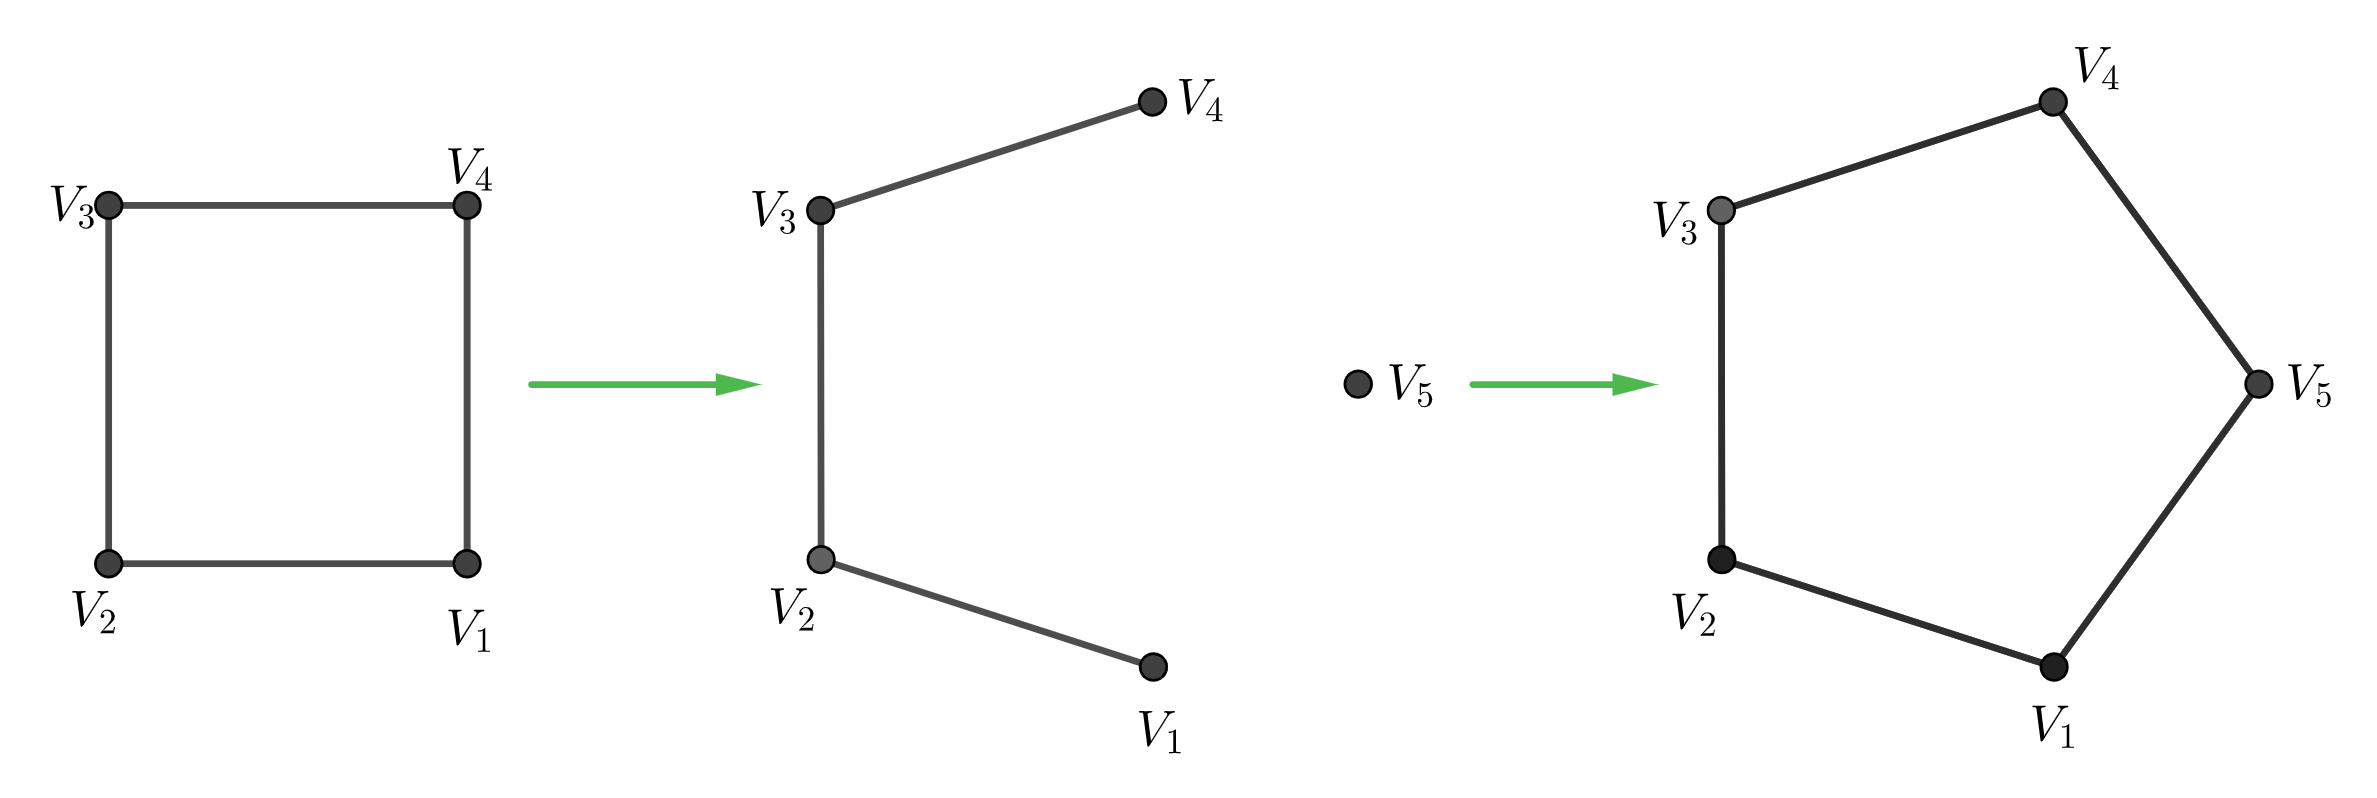
\includegraphics[scale=1]{Imagenes/IMG2/S1-2-04.png}
    \end{center}

    Entonces ahora es más fácil ver que el total de diagonales de un polígono de $n$ lados es el total de diagonales de un polígono de $n-1$ lados más el total de diagonales que van desde el nuevo vértice a los vértices antes dados sumando la diagonal que une a la abertura donde se introdujo el nuevo vértice, estas son $n-2$ diagonales $$D_n= D_{n-1}+(n-2).$$

    Entonces tenemos que 
    \begin{eqnarray*}
        D_n &=& D_{n-1}+(n-2)\\
        &=& D_{n-2}+(n-3)+(n-2)\\
        &=& D_{n-3}+(n-4)+(n-3)+(n-2)\\
        &\cdots& \\
        &=& D_4+(5-2)+(6-2)+\cdots +(n-3)+(n-2)\\
        &=& 2+3+4+\cdots n-2=\dfrac{n(n-3)}{2}.
    \end{eqnarray*}
\end{solucion}
\section{Inclusión-exclusión}

\begin{problema}
¿Cuántos enteros entre 1 y 6300 inclusive, no son divisibles entre 5?
\end{problema}


\begin{problema}
¿Cuántos enteros entre 1 y 6300 inclusive, no son divisibles entre 5 ni entre 3?
\end{problema}


\begin{definicion}
Para calcular la cardinalidad de $A_1\cup A_2\cup\cdots\cup A_n$ se debe calcular la cardinalidad de todas las posibles intersecciones de conjuntos $A_1, A_2,\dots, A_n$ sumar los resultados obtenidos al intersectar un número impar de conjuntos y restar los resultados obtenidos al intersectar un número par de conjuntos.
\end{definicion}

Los términos “inclusión-exclusión” indican que hay que incluir o sumar las cardinalidades de los conjuntos, después excluir o restar las cardinalidades de las intersecciones de dos conjuntos, luego incluir o sumar las cardinalidades de todas las intersecciones de tres conjuntos, etc, es decir:
\[|A_1\cup A_2\cup\cdots\cup A_n|=\sum_{j=1}^{n}(-1)^{j+1}\alpha_j\]

En donde los $\alpha_j$ son las sumas de las cardinalidades de todas las posibles intersecciones de $j$ conjuntos, de la manera siguiente:
\[\alpha_1= |A_1|+|A_2|+|A_3|+\dots+|A_n|\]\[\alpha_2=|A_1\cap A_2|+|A_1\cap A_3|+\dots+|A_{n-1}\cap A_n|\]\[\alpha_3=|A_1\cap A_2\cap A_3|+|A_1\cap A_2\cap A_4|+\dots+|A_{n-2}\cap A_{n-1}\cap A_n|\]...\[\alpha_n=|A_1\cap A_2\cap A_3\cap\dots \cap A_n|\]
En particular:\[|A\cup B| = |A| + |B| - |A\cap B|\]

\begin{problema}
Encuentre $|A\cup B \cup C|$
\end{problema}

\begin{ejemplo}
    Consideremos el conjunto de todas las cadenas de ceros y unos de longitud $10$, ¿cuántas tienen la propiedad de tener por lo menos un 1?
\end{ejemplo}

\begin{solucion}
    Notemos que nos es más simple contar las cadenas que no contienen algún 1, de estas solo es la cadena de puros ceros así si $A$ es el conjunto de todas las cadenas que contienen por lo menos un $1$ y $S$ es el total de cadenas de ceros y unos de longitud 10, tenemos $$S=A\cup \{(00\cdots 0)\},$$ luego $$|A|=|S|-1=2^{10}-1$$.
\end{solucion}


\section{Notación factorial}

Se llama factorial de un número $n\in Z^+$ al producto de los $n$ factores consecutivos desde 1 hasta $n$ y se denota por $n!$. Así:
\[n!=1\times2\times3\times\dots\times(n-2)\times(n-1)\times(n)\]

Aceptaremos que $0!=1$.

\section*{Problemas}

\subsection*{Problemas de interés}

\begin{enumerate}
    \item Usando las letras del conjunto $\{a,b,c,d\}$ ¿de cuantas maneras es posible formar una secuencia ordenada de tres letras en cada uno de los siguientes casos?
    \begin{enumerate}
        \item Si la repetición de letras está permitida.
        \item Si no se permite la repetición de letras.
        \item Sin repetición de letras y que la secuencia tenga a la letra $e$.
        \item Con repetición de letras y conteniendo a la letra $e$.
    \end{enumerate}
    \item ¿Cuántos números entre 1 y 6300 inclusive son divisibles entre 3, entre 5 y entre 7?
    \item De los números entre 1 y 200 ¿Cuántos no son divisibles entre 4, ni entre 6, ni entre 9?
    \item ¿Cuántos números del 1 al 1,000,000 no son ni cuadrados perfectos, ni cubos perfectos, ni potencias cuartas perfectas?
    \item Sea $S$ el conjunto de números de 3 dígitos $abc$ tal que $a,b,c\in \{1,2,\dots,9\}$ y $a,b,c$ son distintos. Encuentre el números de elementos $abc$ en $S$ tal que $a\not=3$, $b\not=5$ y $c\not=7$.
    \item En un grupo de 30 personas, 10 hablan ingles, 12 español y 10 hablan francés. Se sabe que 5 hablan ingles y español, 5 español y francés y 7 ingles y francés. Tres personas hablan los tres idiomas. ¿Cuántas personas no hablan ninguno de estos tres idiomas?
    \item En un grupo hay 100 hindúes hay 40 que hablan hindi, 40 que hablan bengalí y 20 que hablan penjabi. Hay 20 que hablan hindi y bengalí y 5 que hablan hindi y penjabi. Hay 31 que hablan la menos dos de estas lenguas y 33 que no hablan ninguna de ellas. ¿Cuántos hablan las tres lenguas?
    \item Efectúa las siguientes operaciones:
    \begin{multicols}{3}
     \begin{enumerate}
        \item $5!=$
        \item $7!=$
        \item $(8-5)!=$
        \item $8!-5!=$
        \item $4!(5!)=$
        \item $7(8!)-6!=$
    \end{enumerate}   
    \end{multicols}
    

    \item Simplifica las expresiones siguientes:
    \begin{multicols}{3}
        \begin{enumerate}
        \item $\dfrac{8!}{4!}$
        \item $\left(\dfrac{8}{4}\right)!$
        \item $\dfrac{8!}{4}$
        \item $\dfrac{2024!}{2024}$
        \item $\dfrac{7!}{(7-2)!}$
        \item $\dfrac{9!}{3!(9-3)!}$
        \item $\dfrac{12!}{3!(4!)(5!)}$
        \item $\dfrac{4(6!)}{6!(4!)(6)}$
    \end{enumerate}
    \end{multicols}
    \item Halla el valor de $x$ sabiendo que:
    \begin{enumerate}
        \item $x!=110(x-2)!$
        \item $12x! + 5(x+1)!=(x+2)!$
    \end{enumerate}

    \item ¿De cuántas formas diferentes se pueden ordenar las letras de la palabra IMPUREZA?
    \item ¿De cuántas formas se pueden colocar 5 libros diferentes en fila en un mostrador?
\end{enumerate}

\subsection*{Más Problemas}

\begin{enumerate}
    \item Considere una cuadricula $8\times8$. Determine el número de cuadrados formados por vértices de la cuadricula cuyos lados son paralelos a los segmentos de la cuadrícula.

    \item Se dice que en un polígono se ha realizado una triangulación cuando el interior del polígono se cubre con triángulos formados con vértices del polígono de forma tal que los triángulos no se tengan en común más que en conjuntos de puntos de área cero. ¿Cuántos triángulos se requieren en una triangulación en un polígono de $n$ lados?

    \item Cundo se listan los números del 1 al 10000, 'cuántas veces se hace uso del dígito 5? ¿y cuántas veces aparece el 25?

    \item Considere una cuadrícula de $7 \times 7$ 'cuántos rectángulos podemos formar con los vértices de dicha cuadrícula cuyos lados sean paralelos a los segmentos de la cuadrícula?
    
    \item En un campeonato de baloncesto se enfrentan $n$ equipos. En cada ronda los equipos perdedores son eliminados. Si en una ronda el número de equipos aún participando es impar, uno de los equipos, elegido mediante sorteo, descansa y pasa a la siguiente ronda. ¿Cuantos juegos se realizan durante el campeonato?
    \item Se tienen 6 libros distintos de Álgebra, 5 libros distintos de Geometría y 4 libros distintos de Trigonometría. ¿De cuántas formas es posible seleccionar un par de libros tal que no sean de la misma asignatura?
    \item En una circunferencia se marcan 8 puntos. Prueba que el número de triángulos que se pueden formar con vértices en esos puntos es igual al número de pentágonos que se pueden formar con vértices en esos puntos.
    \item Sea $A$ un conjunto finito no vacío. Pruebe que el número de subconjuntos de $A$ con un número par de elementos es igual número de subconjuntos de $A$ con un número impar de elementos.
    \item ¿Cuántos enteros del 1 al 100 no son múltiplos ni de 3 ni de 7?
    \item ¿De cuántas maneras se pueden seleccionar cuatro cartas de un mazo de 52, de modo que haya una cada palo?
    \item ¿De cuántas maneras pueden colocarse una torre blanca y una torre negra en un tablero de
    ajedrez de $8\times 8$ de modo que no se ataquen?
    \item  ¿Cuántos números de tres dígitos tienen el primer dígito impar, el segundo par y el tercero igual a la suma de los dos primeros?
    \item En un acto deben hablar Luis, María, Pedro, Pablo y Luisa. ¿De cuántas maneras se puede confeccionar la lista de oradores? Y si se pone la condición de que se alternen oradores de distinto sexo? ¿Y si la condición es que María hable inmediatamente después que Luis? ¿Y si es que Luis hable antes que Pedro?
    \item ¿Cuántos números naturales tienen exactamente k dígitos?
    \item Para escribir todos los números naturales de k dígitos, ¿cuántos ceros se necesitan?
    \item Para escribir todos los números naturales desde 1 hasta 1000000, ¿cuántos ceros se necesitan?
    \item Los números naturales se escriben uno a continuación del otro: $$1234567891011121314151617181920212223\dotsb$$
    ¿Qué dígito se encuentra en la posición 2023?
    \item  El número 916238457 es un ejemplo de un número de nueve dígitos que contiene cada dígito del 1 al 9 exactamente una vez y cumple con la propiedad de que los dígitos del 1 al 5 aparecen en el orden natural creciente, mientras que los dígitos del 1 al 6 no. ¿Cuántos números existen con estas mismas características?
    
\end{enumerate}